\section{Applications}

\hidenum
\begin{frame}[noframenumbering]
\frametitle{Contents}
 \tableofcontents[currentsection,hideallsubsections]
\end{frame}
\shownum

\subsection{Productivity Example}

\begin{frame}[fragile]
\fontsize{8pt}{10}\selectfont
\begin{block}{Randomized SVD\footnotemark}
  \begin{minipage}{.55\textwidth}
    \begin{center}
      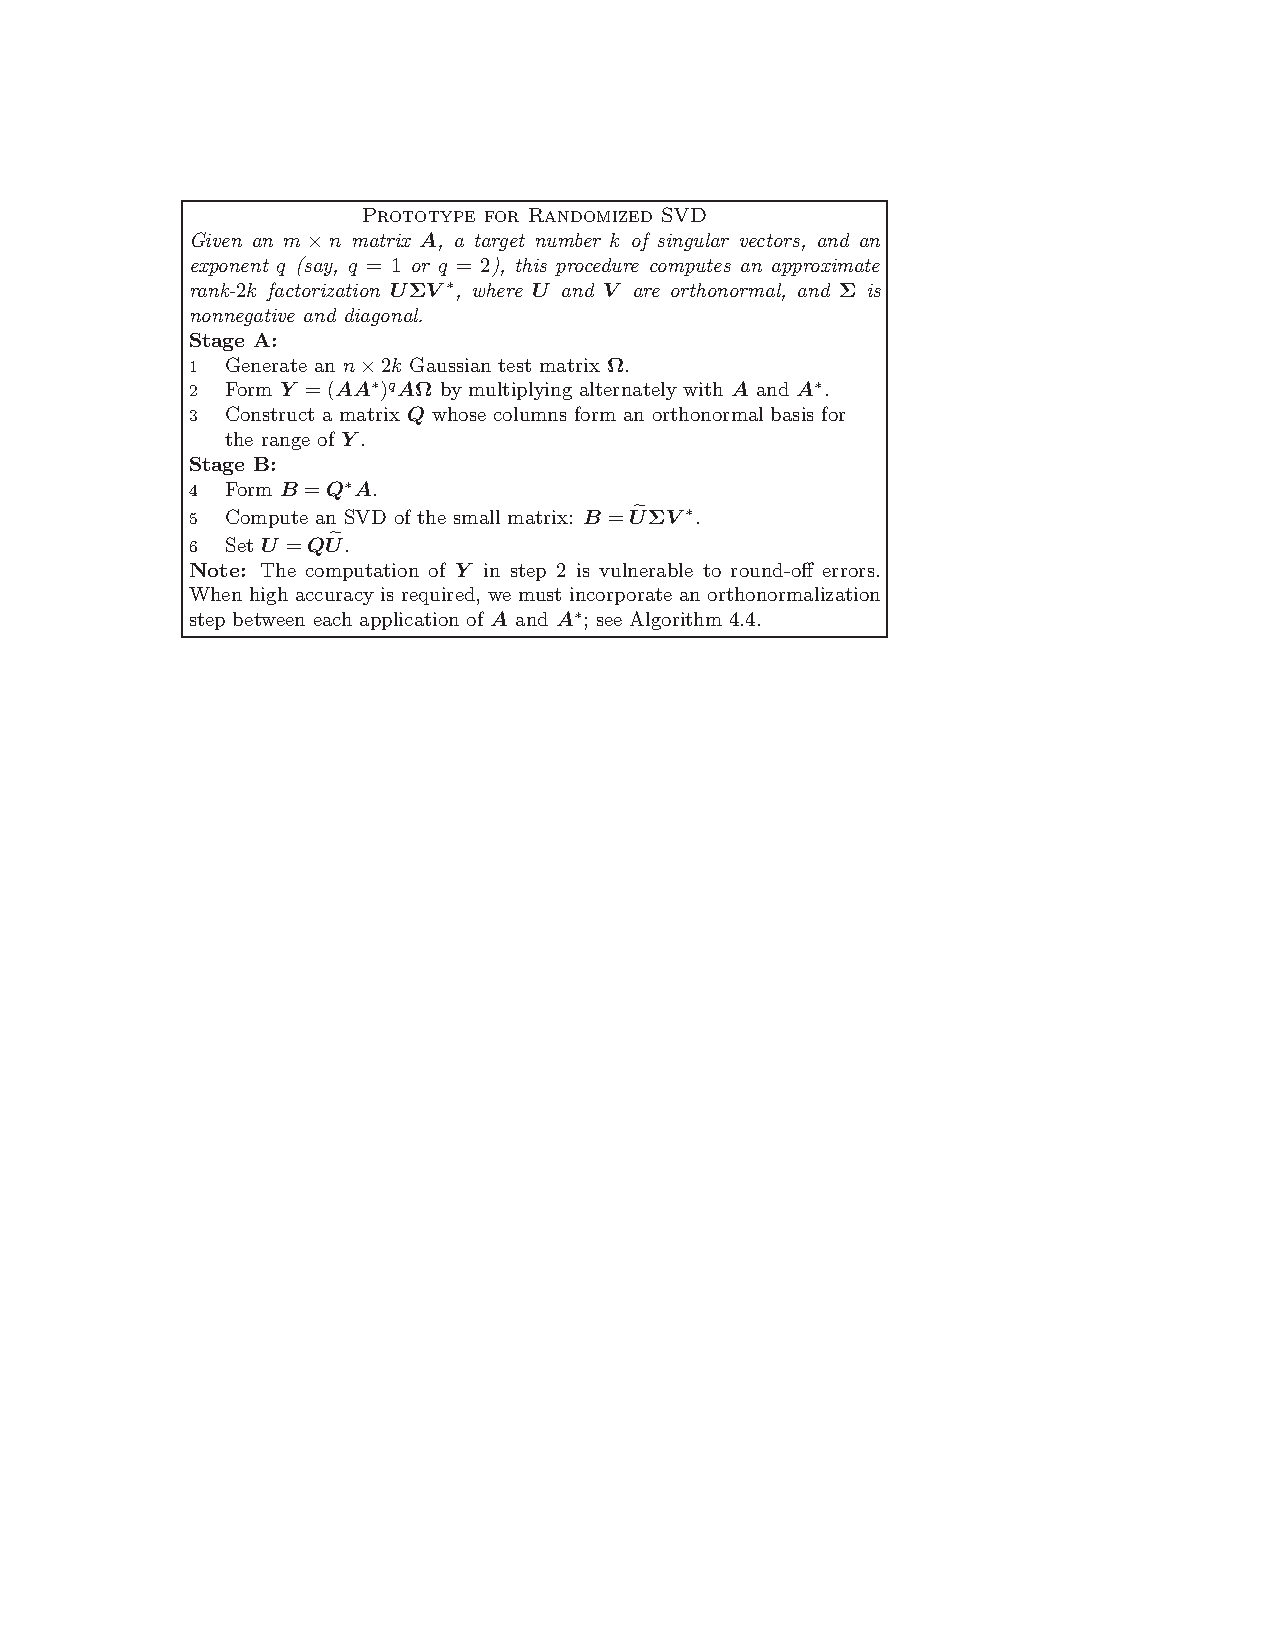
\includegraphics[width=.95\textwidth]{../common/pics/randsvd/randSVDalg}
      \\
      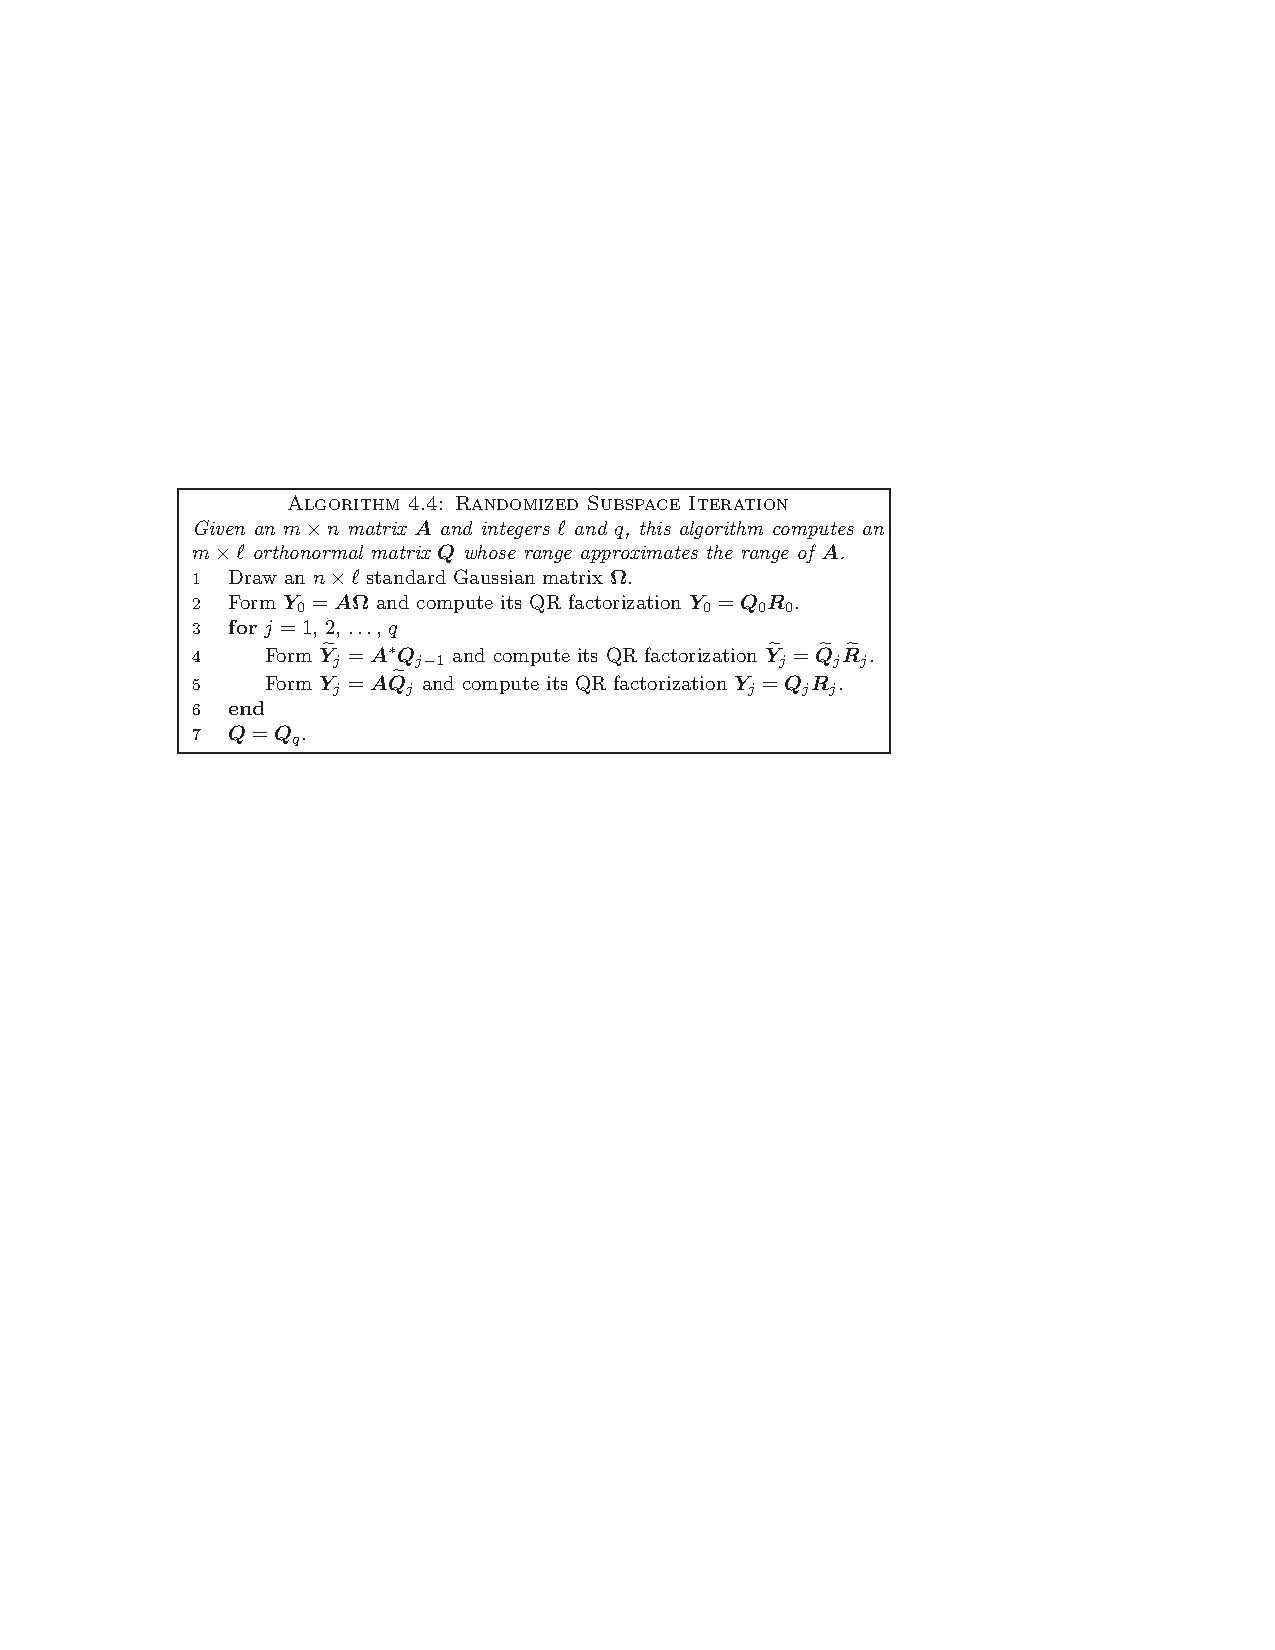
\includegraphics[width=.95\textwidth]{../common/pics/randsvd/randSVDalg4_4}
    \end{center}
  \end{minipage}
%   \hspace{.01cm}
  \begin{minipage}{0.430\textwidth}
\begin{lstlisting}[title=Serial 
R,basicstyle=\tiny,backgroundcolor=\color{grayish} 
,numberstyle=\tiny\color{black},keywordstyle=\color{black},commentstyle=\color{ 
dkgreen},stringstyle=\color{black},escapeinside={(*@}{@*)}]
randSVD <- function(A, k, q=3)
  {
    ## Stage A
    Omega <- (*@ matrix(rnorm(n*2*k),@*) 
            (*@ nrow=n, ncol=2*k) @*)
    Y <- A %*% Omega
    Q <- qr.Q(qr(Y))
    At <- t(A)
    for(i in 1:q)
      {
        Y <- At %*% Q
        Q <- qr.Q(qr(Y))
        Y <- A %*% Q
        Q <- qr.Q(qr(Y))
      }
    
    ## Stage B
    B <- t(Q) %*% A
    U <- La.svd(B)$u
    U <- Q %*% U
    U[, 1:k]
  }
\end{lstlisting} %balance$
\end{minipage}
{\fontsize{6pt}{10}\selectfont $^1$Halko N, Martinsson P-G 
  and Tropp J A 2011 Finding structure with randomness: probabilistic algorithms 
  for constructing approximate matrix decompositions \emph{SIAM Rev.} \textbf{53} 
  217--88}
\end{block}
\end{frame}


\begin{frame}[fragile]
 \fontsize{8pt}{10}\selectfont
\begin{block}{Randomized SVD}
  \hfill
  \begin{minipage}{0.430\textwidth}
\begin{lstlisting}[title=Serial 
R,basicstyle=\tiny,backgroundcolor=\color{grayish} 
,numberstyle=\tiny\color{black},keywordstyle=\color{black},commentstyle=\color{ 
dkgreen},stringstyle=\color{black},escapeinside={(*@}{@*)}]
randSVD <- function(A, k, q=3)
  {
    ## Stage A
    Omega <- (*@ \textcolor{blue}{matrix(rnorm(n*2*k),} @*) 
         (*@ \textcolor{blue}{ nrow=n, ncol=2*k)} @*)
    Y <- A %*% Omega
    Q <- qr.Q(qr(Y))
    At <- t(A)
    for(i in 1:q)
      {
        Y <- At %*% Q
        Q <- qr.Q(qr(Y))
        Y <- A %*% Q
        Q <- qr.Q(qr(Y))
      }
    
    ## Stage B
    B <- t(Q) %*% A
    U <- La.svd(B)$u
    U <- Q %*% U
    U[, 1:k]
  }
\end{lstlisting} %balance$
  \end{minipage}
  \hfill
  \begin{minipage}{0.430\textwidth}
\begin{lstlisting}[title=Parallel pbdR,basicstyle=\tiny,backgroundcolor=\color{
grayish}, numberstyle=\tiny\color{black},keywordstyle=\color{black},
commentstyle=\color{dkgreen},stringstyle=\color{black},escapeinside={(*@}{@*)}]
randSVD <- function(A, k, q=3)
  {
    ## Stage A
    Omega <- (*@ \textcolor{blue}{ddmatrix("rnorm",} @*)
         (*@ \textcolor{blue}{nrow=n, ncol=2*k)} @*)
    Y <- A %*% Omega
    Q <- qr.Q(qr(Y))
    At <- t(A)      
    for(i in 1:q)
      {
        Y <- At %*% Q   
        Q <- qr.Q(qr(Y))
        Y <- A %*% Q    
        Q <- qr.Q(qr(Y))
      }
    
    ## Stage B
    B <- t(Q) %*% A     
    U <- La.svd(B)$u 
    U <- Q %*% U     
    U[, 1:k]
  }
\end{lstlisting}  % balancing $
  \end{minipage}
\hfill
\end{block}
\end{frame}

\begin{frame}
  \begin{block}{Randomized SVD on $\approx 765$ MiB}
    \begin{center}
      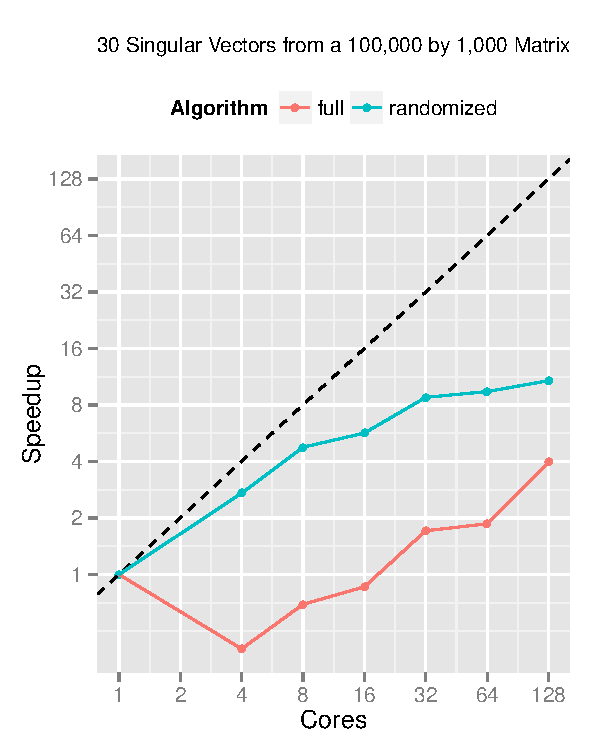
\includegraphics[width=.45\textwidth]{../common/pics/randsvd/randSVDspeedup}
      \hfill
      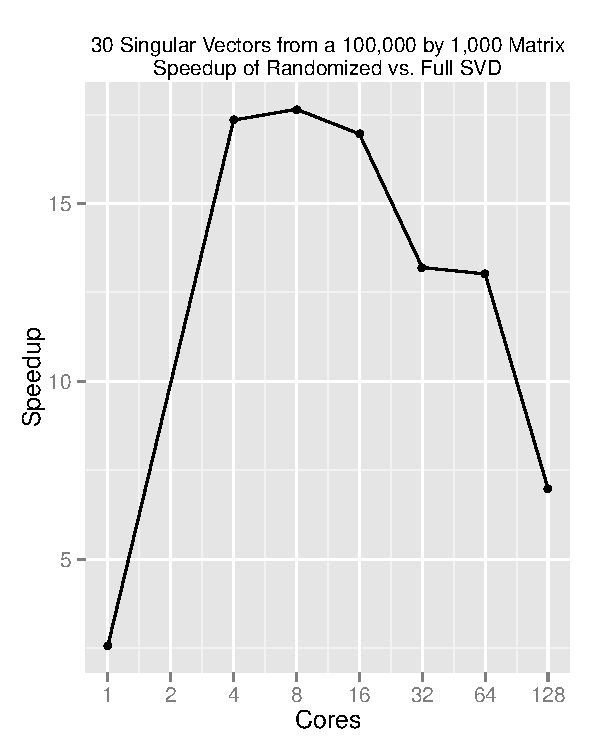
\includegraphics[width=.45\textwidth]{../common/pics/randsvd/randSpeedupSVD}
    \end{center}
  \end{block}
\end{frame}

\subsection{Science Applications}

\begin{frame}
  \begin{block}{\scriptsize Exploration of Climate Data (2.9 TB) with pbdR} 
    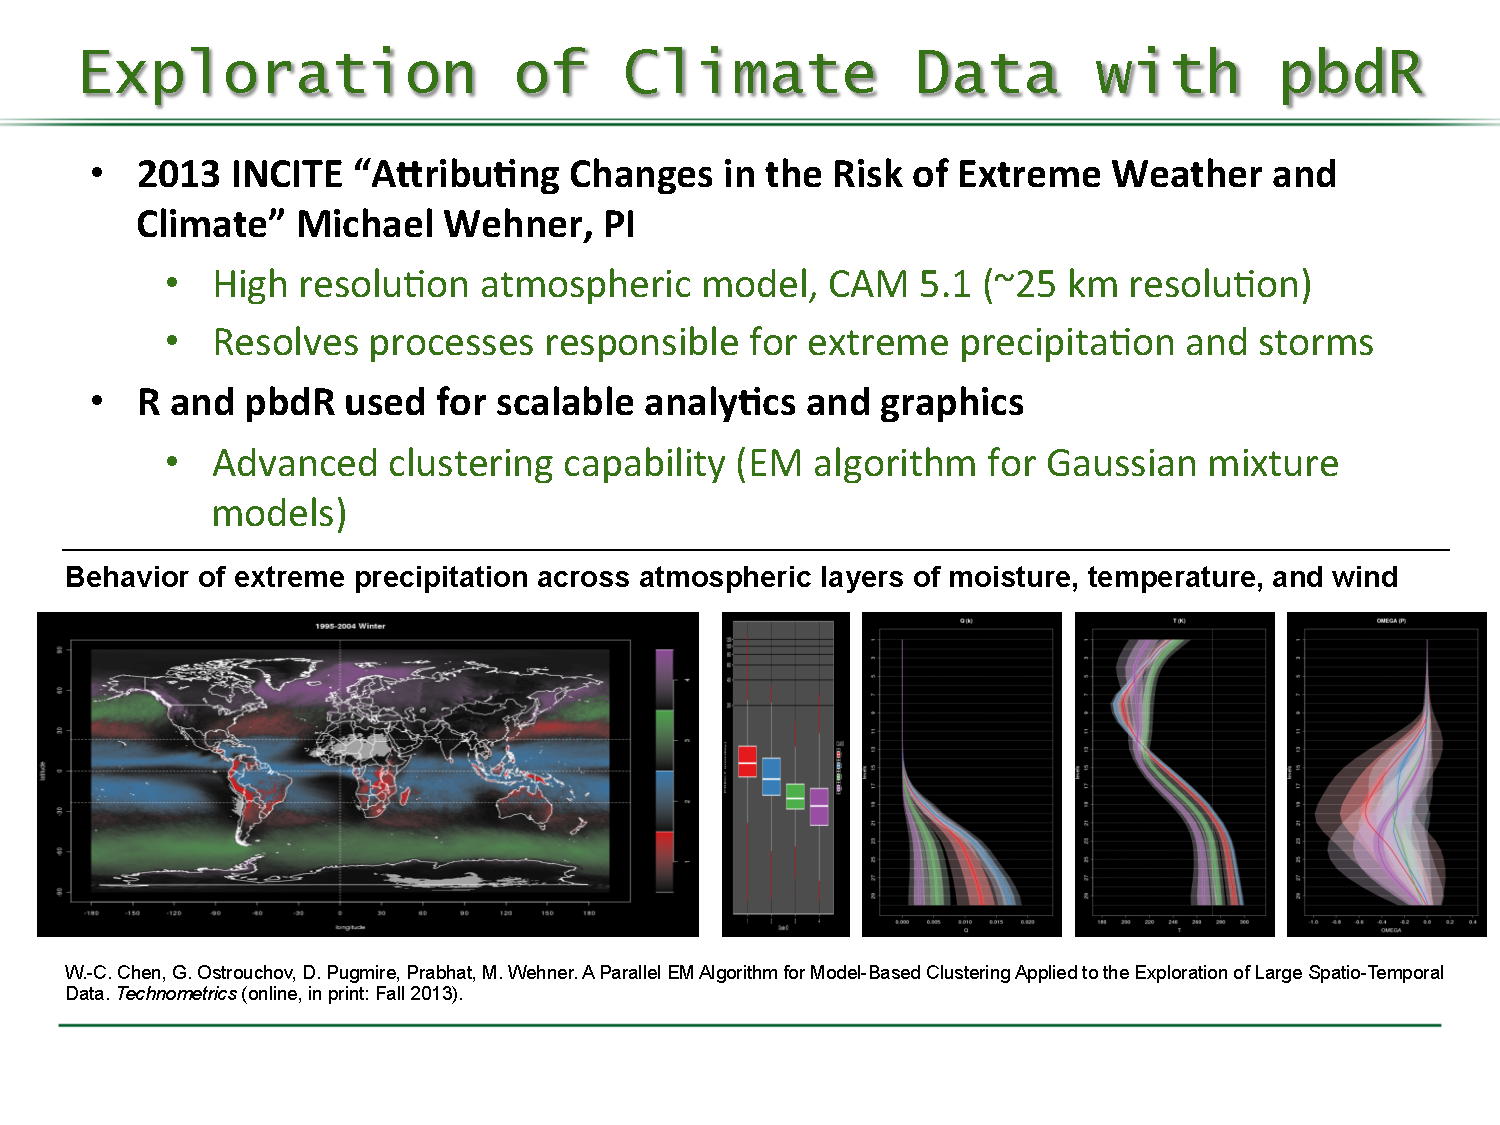
\includegraphics[width=\textwidth,trim=0ex 9ex 0ex 13ex,clip]{../common/pics/apps/ClimateApp.pdf}
  \end{block}
\end{frame}

\begin{frame}
  \begin{block}{Simulation in the Social Sciences with \pbdR}
  \begin{minipage}[b]{.88\textwidth}
  \begin{itemize}\small
    \item Survey responses can be intentionally misleading
    \item This results in bias and poor policy decisions
    \item Simulation examines bias
    \end{itemize}
  \end{minipage}
  \begin{minipage}[b]{.10\textwidth}
    
\includegraphics[scale=0.13]{../common/pics/survey}\vspace{.2cm}
  \end{minipage}
  \emph{``$\ldots$ [Serial] simulations would require {\bf nearly a
      year} to complete. $\ldots$ Using [\pbdR] and NICS resources,
    {\bf the simulation completed in just 15 hours}.''} \\
 --- Joseph Robinson, Educational Psychology, University of Illinois at
  Urbana-Champaign
  \end{block}

  \begin{block}{Engaging with the R Community}
    \emph{``It's exactly what I wanted ever since I started learning about HPC 
      with C and MPI a few years back!''} \\ --- Andrew Raim,
    Department of Mathematics and Statistics, University of Maryland, 
    Baltimore County
  \end{block}
\end{frame}

\begin{frame}
  \begin{block}{Coherent Structures in Turbulent Flow with \pbdR} 
    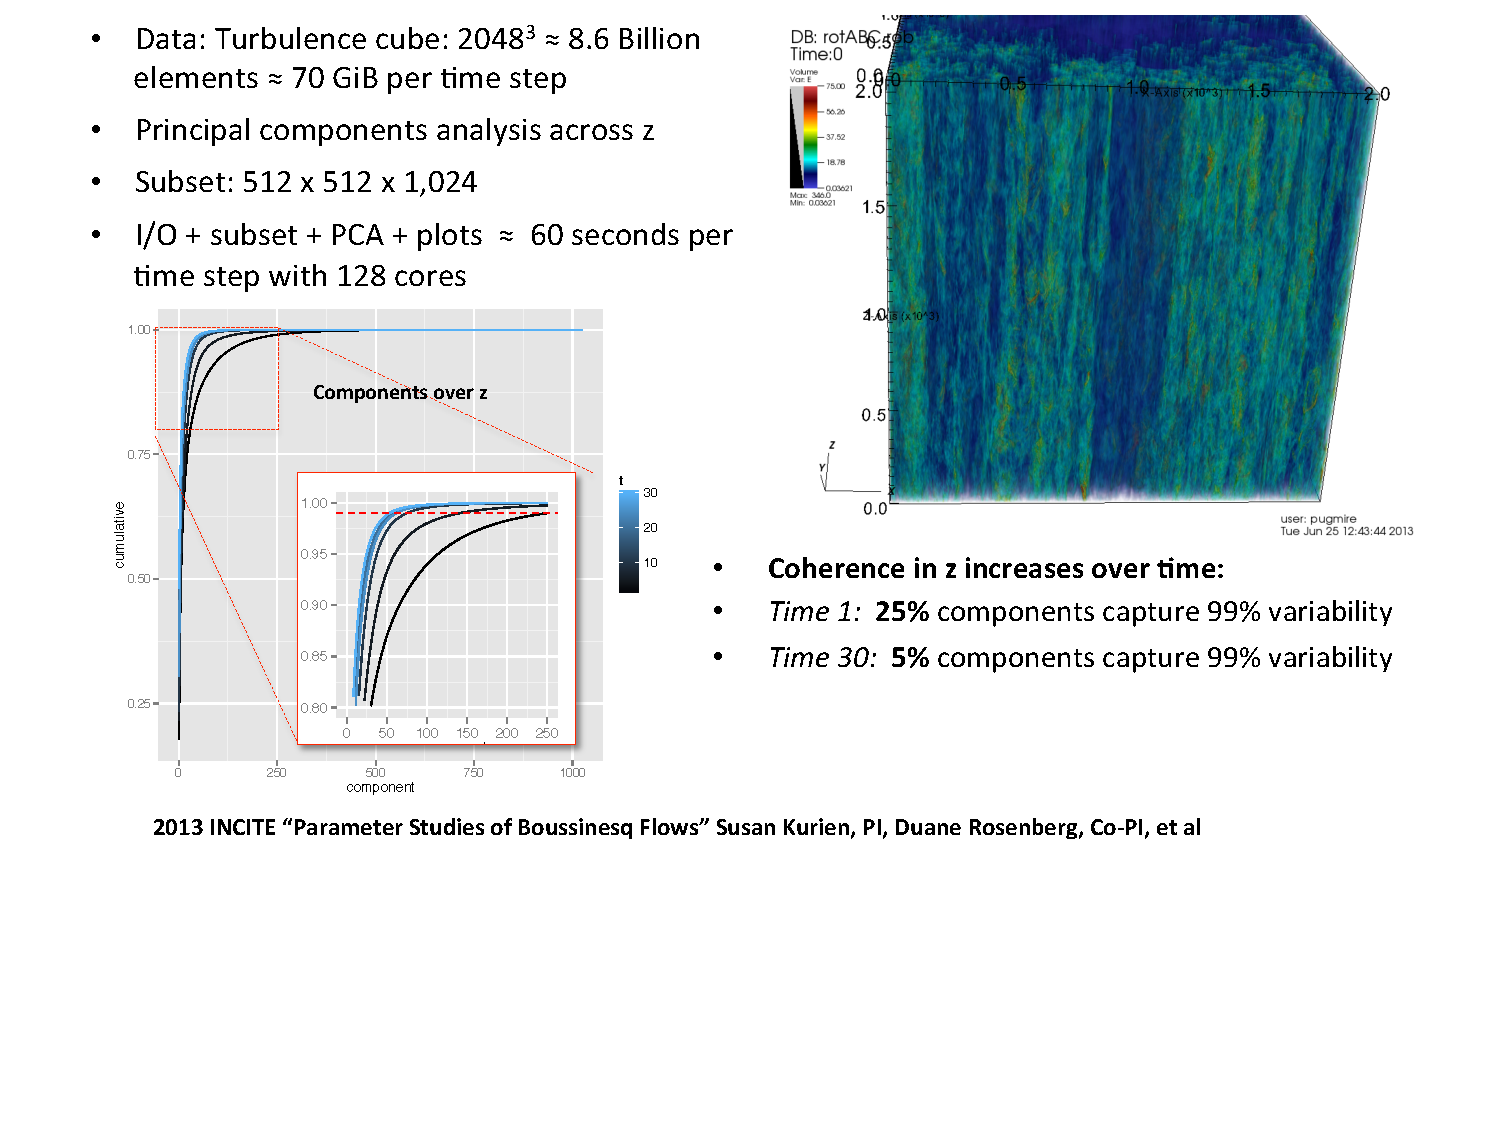
\includegraphics[width=\textwidth,trim=8ex 28ex 8ex 0ex,clip]{../common/pics/apps/TurbulentFlowINCITE.pdf}
  \end{block}
\end{frame}


